\documentclass[11pt,a4paper]{article}
\usepackage[margin=2.2cm]{geometry}
\usepackage[T1]{fontenc}
\usepackage{lmodern}
\usepackage{amsmath,amssymb}
\usepackage{graphicx}
\usepackage{booktabs}
\usepackage{float}
\usepackage{caption}
\usepackage{longtable}
\usepackage{adjustbox}
\usepackage{xcolor}
\usepackage[colorlinks=true,linkcolor=blue!50!black,citecolor=blue!50!black,urlcolor=blue!50!black]{hyperref}

\captionsetup{font=small,labelfont=bf}
\newcommand{\sxy}{\sigma_{xy}}
\newcommand{\keV}{\,\mathrm{keV}}
% table bodies are read with the TeX primitive \input: LaTeX's \input (with file hooks, 2020+) is not
% expandable, which puts the \bottomrule after it out of place ("Misplaced \noalign")
\makeatletter\newcommand{\tabinput}[1]{\@@input #1 }\makeatother

\title{Am-241 lines in the AMtest skipper-CCD data:\\
gain-vs-charge correction, cluster-width cut and a constrained fit of the 10--30\,keV region}
\author{Dylan Rosenmerkel}
\date{\today}

\begin{document}
\maketitle

\begin{abstract}
We analyse 29 Am-241 exposures (Image~8, ACM board~106, CCDs EXT1, EXT3, EXT4) taken between
2026-03-30 and 2026-05-26. Two steps are needed to see the low-energy Am-241 lines at the right energies.
(i) A gain-vs-charge correction, with the gain curve $g(n)$ measured from the images themselves, moves the
59.54\,keV peak on EXT4 from 0.932 to 0.992 of its true energy. The gain stepped down by 1--5\,\% between images
\#40 and \#41, so one curve per CCD and gain period is used. (ii) A cut on the cluster width, $\sxy<0.7$\,pixels,
removes most of the continuum under the 10--30\,keV lines. A binned Poisson-likelihood fit of 10--30\,keV with
the Np L-line energies and intensity ratios of L\'epy et al.~\cite{lepy2008} then finds on EXT4 the Np L$\beta$,
L$\gamma$ and L$\alpha$ groups at 15.5, 16.0 and 4.0 standard deviations, the 26.3\,keV $\gamma$ ray at
14.8$\sigma$, with all lines on a common energy scale $k = 0.9840 \pm 0.0008$. Without the cut, the fit cannot
separate the lines. Two additional lines at $22.11\keV$ and $24.93\keV$, which do not come from the Am-241 decay,
are also required; they are attributed to silver K fluorescence (to be confirmed), e.g.\ from the silver backing
typical of smoke-detector americium foils.
\end{abstract}

\tableofcontents

%======================================================================
\section{Summary of results}
\begin{itemize}
\item \textbf{Figure of merit:} the constrained 10--30\,keV fit on EXT4 after the cut,
Fig.~\ref{fig:fit}, with its fit parameters in Table~\ref{tab:fitpar} and the fitted peak centroids, widths and
FWHM in Table~\ref{tab:groups}. Deviance/ndf is 1.74; the pulls (Sec.~\ref{sec:pulls}) scatter with an RMS of 1.22
and show one localised excess at 24.0--25.2\,keV.
\item \textbf{Energy scale:} the 10--30\,keV lines sit at $k = 0.9840 \pm 0.0008$ of their tabulated
energies after the gain correction ($0.9358$ without it). The 59.54\,keV $\gamma$ ray is at 0.994 and the Fe-55
Mn K$\alpha$ line at 0.996.
\item \textbf{Gain correction:} needed to put the peaks at the right energies and to remove the image-to-image
scatter of the per-image fitted gain (Sec.~\ref{sec:gain}). A gain step between images \#40 and \#41
requires one $g(n)$ curve per gain period.
\item \textbf{Width cut:} $\sxy<0.7$\,pixels, chosen with a fit-based figure of merit on a grid of lower and
upper limits and checked on independent halves of the images (Sec.~\ref{sec:cut}). Lower limits do not help.
\item \textbf{Other peaks} (Sec.~\ref{sec:other}): the Compton edge of the 59.54\,keV $\gamma$ ray at
$10.82 \pm 0.06\keV$, the backscatter peak at $49.28 \pm 0.13\keV$, and Fe-55 Mn K$\alpha$/K$\beta$ lines.
\item \textbf{Silver K lines (to be confirmed)} at $22.112\pm0.037$ and $24.933\pm0.060\keV$ (408 and 202
counts) are needed to describe the data (Sec.~\ref{sec:extra}). They are not Am-241 photons, conversion electrons
or Am self-fluorescence, and an enhanced Np L$\gamma_4$ is disfavoured. Both energies match Ag K$\alpha$/K$\beta$, and
smoke-detector americium foils commonly have a silver backing; the intensity ratio (0.49) is higher than expected
for silver and still has to be explained.
\end{itemize}

%======================================================================
\section{Data and processing}
\label{sec:data}
The data are 29 images (\#21 and \#23--\#50; Image~8, ACM board~106) of the AMtest Am-241 run.
Each image has four CCD extensions; EXT2 was flagged by the pipeline as flooded/unresolved on every image and is not
used. EXT4 has by far the most Am-241 clusters (154\,658 in total, against 73\,793 on EXT3 and 46\,508 on EXT1), and
the results below are for EXT4 unless stated otherwise.

The images were processed with \texttt{run\_WADERs} (\texttt{comm\_scripts}), which
\begin{enumerate}
\item builds one panaSKImg configuration per CCD from the raw pixels (pedestal method, gain from a fit of
the 0\,e$^-$/1\,e$^-$ peaks or of all resolved electron peaks, dark current);
\item runs panaSKImg (WADERs) once per CCD, including cluster finding, and collects the cluster files
(\texttt{panaSKImg\_clustersRec\_<image>\_ext<N>.root});
\item with \texttt{--gain-correction}, measures the gain vs charge per pixel $g(n)$ and writes corrected cluster
files (Sec.~\ref{sec:gain});
\item with \texttt{--composite}, runs \texttt{MakeComposite\_Fe55\_Clusters\_Extensions.cc} on the cluster
files (composite clusters, Fe-55 fits, Am-241 spectra).
\end{enumerate}
The cluster energy is the sum over its pixels of the charge in electrons times 3.74\,eV. The analysis below
uses the per-cluster quantities of the cluster files: energy, the fitted widths $\sigma_x,\sigma_y$
(\texttt{fSTD\_X}, \texttt{fSTD\_Y}), the charge-weighted RMS \texttt{wSTD\_XY}, the brightest-pixel charge,
the number of pixels, PCA shape variables, the distance to the nearest cluster and the position.

%======================================================================
\section{Gain-vs-charge correction}
\label{sec:gain}
\subsection{Why it is needed}
panaSKImg converts ADU to electrons with one gain per CCD and image, fitted on the 0\,e$^-$ and 1\,e$^-$ peaks.
Two effects make that conversion wrong for keV clusters: the gain falls with the charge in a pixel (2--4\,\%
lower at 1000\,e$^-$, Table~\ref{tab:curves}), so pixels with hundreds to thousands of electrons are converted to
too few electrons and the line energies come out low; and the fitted low-charge gain scatters from image to image
(rms 0.4--0.9\,\% within a gain period on EXT3/EXT4, about 4\,\% on EXT1, where the 1\,e$^-$ peak is weak), which shifts each image's peaks
differently and broadens the summed peaks.

\subsection{Method}
\texttt{gain\_vs\_charge.py} measures $g(n)$, the local gain at $n$ electrons, from the spacing of the electron
comb in the pixel-charge distribution of clean rows (a periodogram at increasing charge), adding the comb power of all
images of a CCD. The default model is a monotone cubic (PCHIP) interpolation through the measured points; above the
highest measured charge $n_\mathrm{max}$ it continues linearly to $3\,n_\mathrm{max}$ and is constant beyond.
Each pixel's ADU value is converted to electrons by inverting $\mathrm{ADU}(n)=\int_0^n g(n')\,dn'$, and the cluster
energies are recomputed. The low-charge gain $g(0)$ of the curve is used for every image of the group, so the
image-to-image scatter of the fitted 0\,e$^-$/1\,e$^-$ gain is removed as well.

\subsection{A gain step between images \#40 and \#41}
With one curve per CCD for all 29 images, images \#41--\#50 (2026-05-21 to 05-26) came out about 3\,\% low on EXT4
(Fig.~\ref{fig:stability}, grey). The per-image fitted gain confirms a step: compared with images \#21--\#40 it is
lower by 2.8\,\% on EXT3 (1.3113 $\to$ 1.2750\,ADU/e$^-$), 1.3\,\% on EXT4 and 4.8\,\% on EXT1, and stable within
each period (rms 0.4\,\% on EXT3). The comb measurement sees the same step in $g(0)$
(Table~\ref{tab:curves}, Fig.~\ref{fig:curves}). We therefore measure and apply one curve per CCD and \emph{gain period}
(images \#21--\#40 and \#41--\#50). On EXT1 the second period gives no reliable curve and those files are left
uncorrected; EXT1 is not used for the line fits.

\begin{table}[H]
\centering
\caption{Gain curves per CCD and gain period: low-charge gain $g(0)$ of the comb curve, the mean per-image
0\,e$^-$/1\,e$^-$ gain fitted by panaSKImg, the drop of $g(n)$ at 1000\,e$^-$ and the highest charge at which $g$
was measured (above it the curve is extrapolated).}
\label{tab:curves}
\begin{adjustbox}{max width=\textwidth}
\begin{tabular}{llcccc}
\toprule
images & CCD & $g(0)$ [ADU/e$^-$] & fitted gain [ADU/e$^-$] & drop at 1000\,e$^-$ [\%] & $n_\mathrm{max}$ [e$^-$] \\
\midrule
\tabinput{tables/gain_curves.tex}
\bottomrule
\end{tabular}
\end{adjustbox}
\end{table}

\begin{figure}[H]
\centering
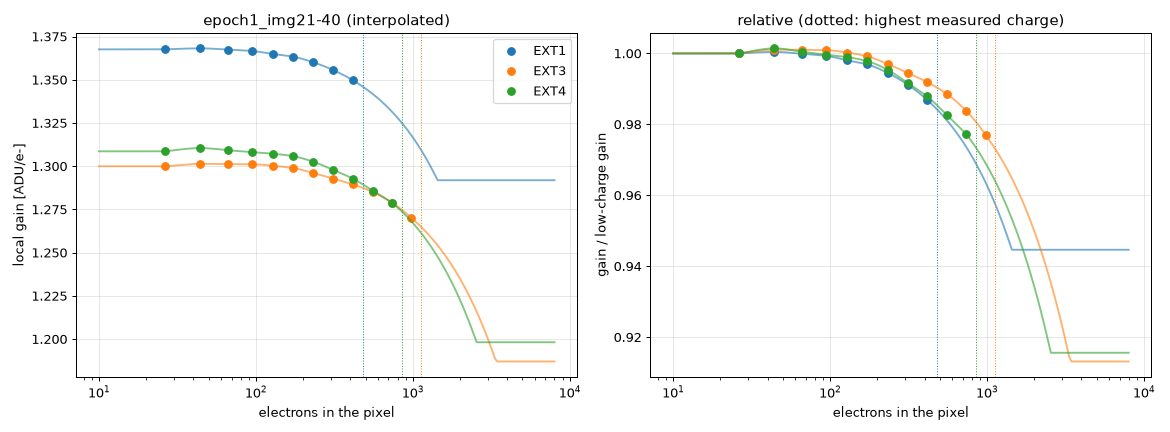
\includegraphics[width=0.49\textwidth]{figures/gain_curve_img21-40.png}\hfill
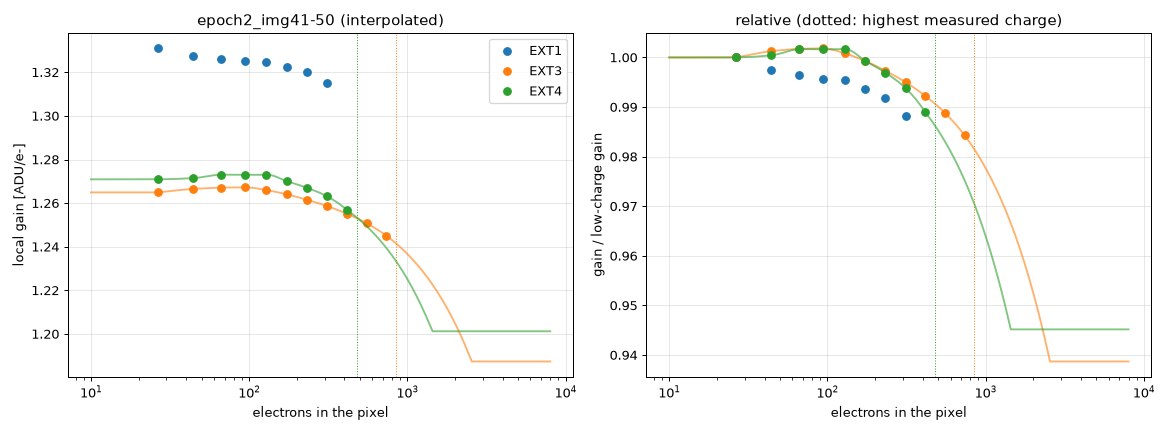
\includegraphics[width=0.49\textwidth]{figures/gain_curve_img41-50.png}
\caption{Gain vs charge per pixel $g(n)$ for images \#21--\#40 (left) and \#41--\#50 (right). Points: measured
local gain; lines: the interpolated model. In each panel the left plot is $g(n)$ in ADU/e$^-$, the right one
$g(n)/g(0)$; dotted lines mark the highest measured charge.}
\label{fig:curves}
\end{figure}

\subsection{Effect on the 59.54\,keV peak}
Table~\ref{tab:gain595} and Figs.~\ref{fig:peak595} and \ref{fig:stability} compare no correction, one curve for all
images, and one curve per gain period. Without correction the EXT4 peak sits 6.8\,\% low and is 0.92\,keV wide
(Gaussian $\sigma$). With one curve per period all images line up: the image-by-image peak positions scatter by
0.25\,\% (EXT4) and 0.18\,\% (EXT3) around 0.992 and 0.998 of the true energy. With one curve for all images, the
summed EXT4 peak splits in two (Fig.~\ref{fig:peak595}); its quoted width of 0.351\,keV in
Table~\ref{tab:gain595} is that of the larger sub-peak only, because the Gaussian fit locks on the images
\#21--\#40 peak and treats the images \#41--\#50 peak as background. The per-period value, 0.473\,keV, is the
honest width of the summed peak.

\begin{table}[H]
\centering
\caption{59.54\,keV peak position (fitted mean / 59.54\,keV) for the two gain periods and for all 29 images, and the
Gaussian $\sigma$ of the summed peak. All clusters; Gaussian plus linear background fitted from 1.2\,keV below to
1.5\,keV above the maximum.}
\label{tab:gain595}
\begin{adjustbox}{max width=\textwidth}
\begin{tabular}{llcccc}
\toprule
CCD & correction & images 21--40 & images 41--50 & all & $\sigma$ all [keV] \\
\midrule
\tabinput{tables/gain_595.tex}
\bottomrule
\end{tabular}
\end{adjustbox}
\end{table}

\begin{figure}[H]
\centering
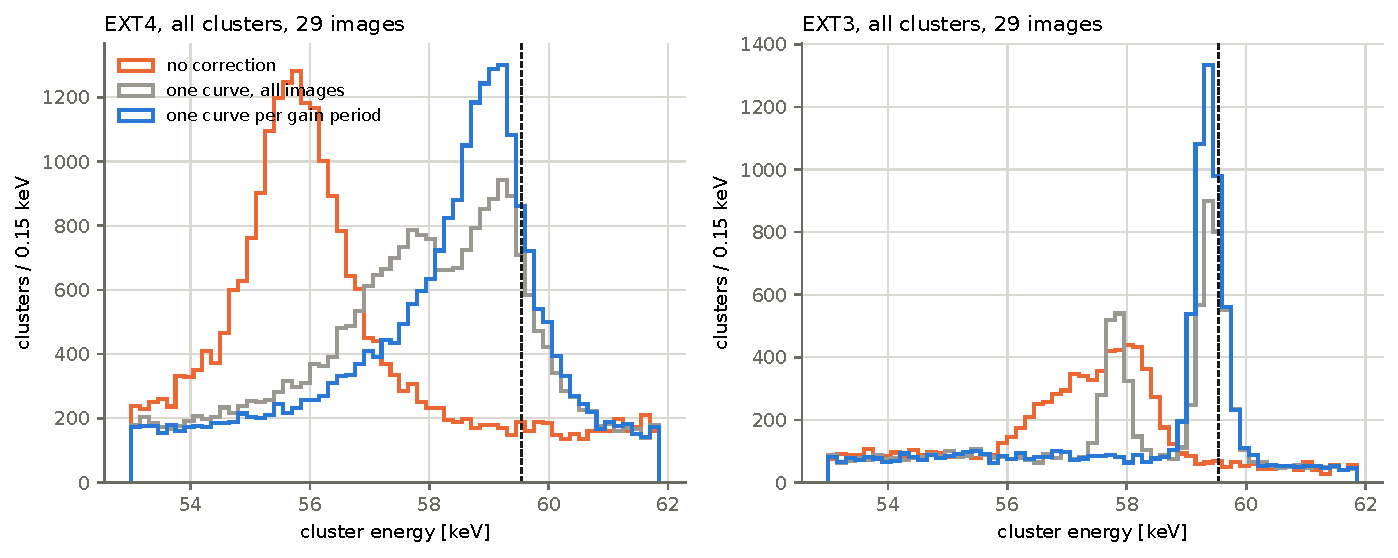
\includegraphics[width=\textwidth]{figures/peak595_versions.pdf}
\caption{The 59.54\,keV peak (all clusters, all 29 images) without correction, with one $g(n)$ curve for all
images, and with one curve per gain period. The dashed line is the true energy.}
\label{fig:peak595}
\end{figure}

\begin{figure}[H]
\centering
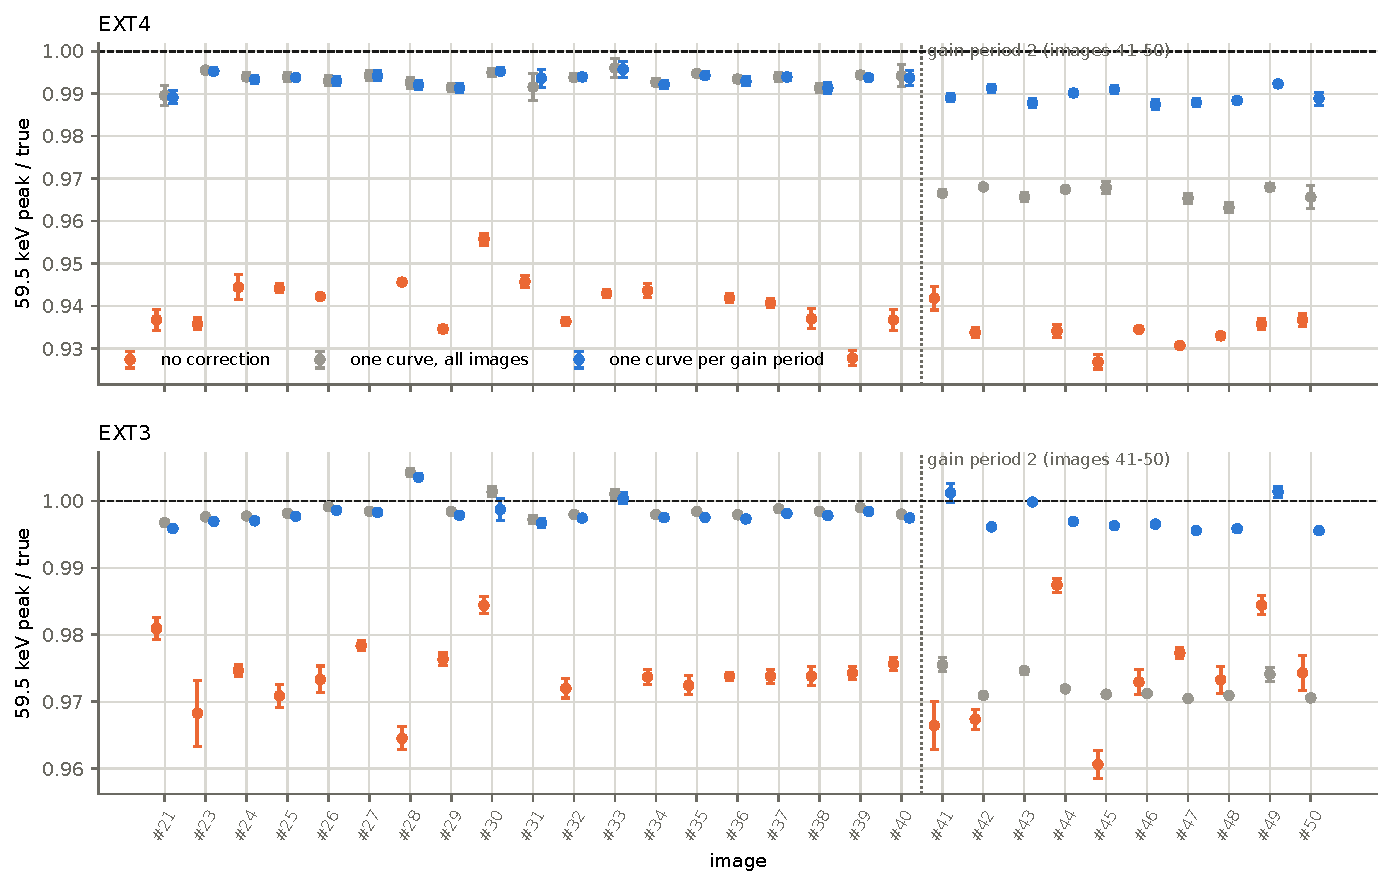
\includegraphics[width=\textwidth]{figures/stability595.pdf}
\caption{59.54\,keV peak position image by image (fitted on each image alone; missing points: no clean peak in that
image). The dotted line marks the gain step between images \#40 and \#41.}
\label{fig:stability}
\end{figure}

%======================================================================
\section{Cluster-width cut}
\label{sec:cut}
\subsection{Definition}
The cluster width is
\begin{equation}
\sxy = \sqrt{\tfrac12\left(\sigma_x^2+\sigma_y^2\right)},
\end{equation}
where $\sigma_x$ and $\sigma_y$ are the widths of Gaussian fits to the cluster's projections on the columns and rows
(panaSKImg \texttt{fSTD\_X}, \texttt{fSTD\_Y}), the same quantity \texttt{MakeComposite} uses for its
front/back split.

\subsection{Motivation}
The charge of an interaction diffuses on its way to the pixels; the further it drifts, the wider the cluster.
Low-energy x rays are absorbed close to the surface they enter (attenuation length in silicon of order 0.5\,mm at
15\,keV and 1\,mm at 20\,keV), while the 59.54\,keV $\gamma$ ray converts almost uniformly in depth (of order
13\,mm). The continuum under the L lines (Compton scatters of the 59.54\,keV $\gamma$ ray and partially collected
59.54\,keV interactions) is spread over all widths. Figure~\ref{fig:width}: the L lines appear as vertical stripes
at small width (left); clusters in the L$\beta$, L$\gamma$ and 26.3\,keV windows are mostly below
$\sxy\approx 0.7$, the neighbouring continuum mostly above (middle).

Wide clusters also lose charge, because the faint edges of a diffuse cluster fall below the pixel threshold. In
slices of width the fitted energy scale of the 10--30\,keV lines drops from 0.991 ($\sxy<0.33$) to 0.931
($0.8\le\sxy<1.0$) (Table~\ref{tab:slices}, Fig.~\ref{fig:width} right). A loose width cut therefore mixes clusters
with different energy scales and smears the lines; this, not only the larger background, limits how far the cut can
be opened.

\begin{figure}[H]
\centering
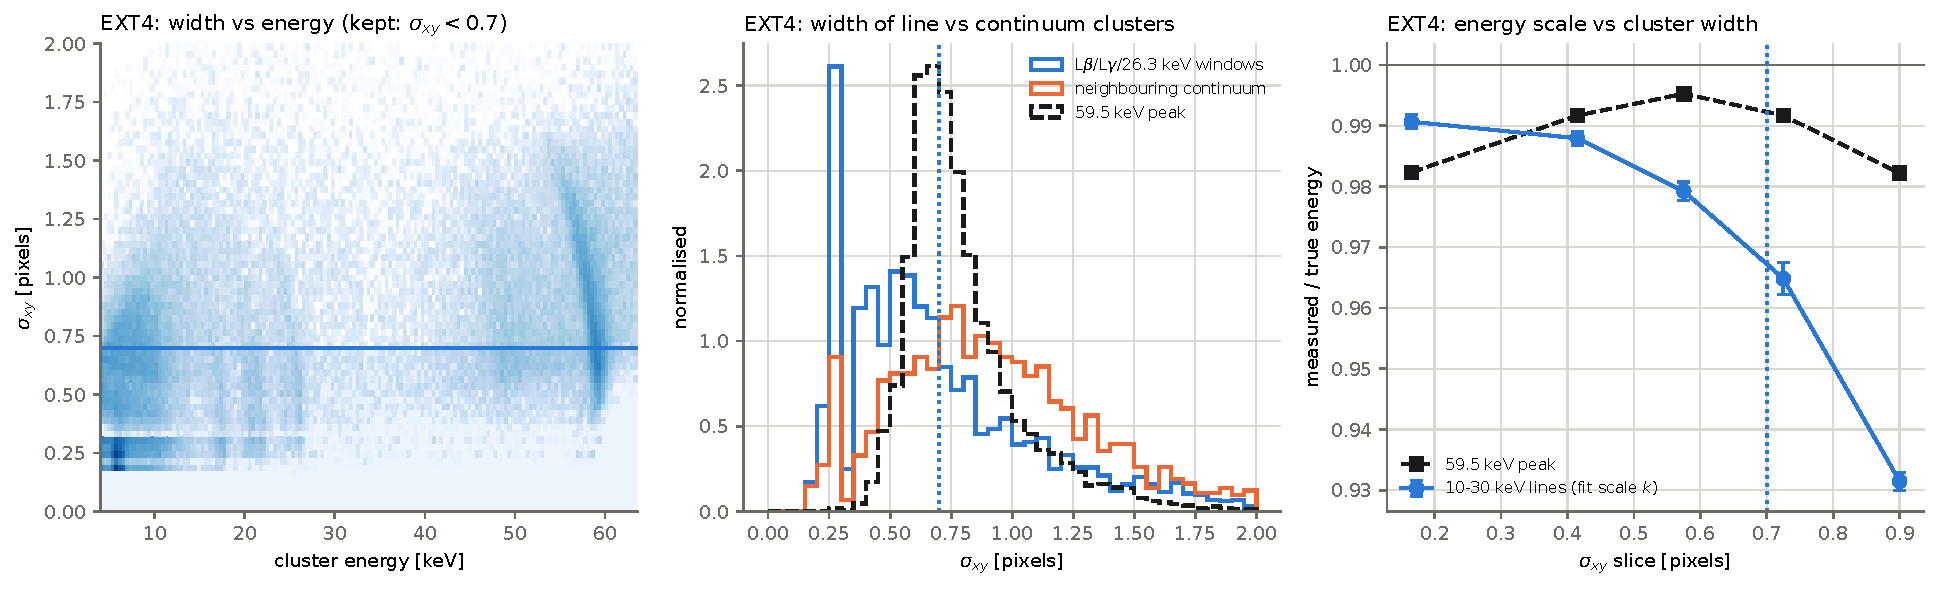
\includegraphics[width=\textwidth]{figures/width_motivation.pdf}
\caption{EXT4, gain-corrected. Left: cluster width vs energy; the band below the line is kept. Middle: width of the
clusters in the L$\beta$/L$\gamma$/26.3\,keV windows, in the neighbouring continuum and in the 59.54\,keV peak.
Right: energy scale vs width: fit scale $k$ of the 10--30\,keV lines and the 59.54\,keV peak position, in slices of
$\sxy$.}
\label{fig:width}
\end{figure}

\begin{table}[H]
\centering
\caption{EXT4, gain-corrected: the constrained fit (Sec.~\ref{sec:fit}) in slices of cluster width. The scale of
the 10--30\,keV lines falls with width. The 59.54\,keV value in the narrowest slice rests on few events (few
59.54\,keV $\gamma$ rays convert close enough to the surface).}
\label{tab:slices}
\begin{adjustbox}{max width=\textwidth}
\begin{tabular}{ccccc}
\toprule
$\sxy$ [pixels] & clusters & scale $k$ (10--30\,keV) & L$\beta$ significance & 59.54\,keV / true \\
\midrule
\tabinput{tables/width_slices.tex}
\bottomrule
\end{tabular}
\end{adjustbox}
\end{table}

\subsection{Quantisation of $\sxy$}
For clusters only 1--3 pixels wide the Gaussian fits of the projections have 1--3 non-empty bins, and the fitted
width depends almost only on how many pixels the cluster spans: about 0.19 for one pixel, 0.25--0.30 for two pixels
(it cannot exceed $\approx 0.30$ however the charge is shared), and $\ge 0.33$ for three. This produces the spikes
and the near-empty band at $\sxy=0.30$--$0.33$ in Fig.~\ref{fig:quant}. The compact clusters are real L x rays;
only their width value is quantised. The charge-weighted RMS \texttt{wSTD\_XY} is continuous and gives the same
results (Table~\ref{tab:band}).

\begin{figure}[H]
\centering
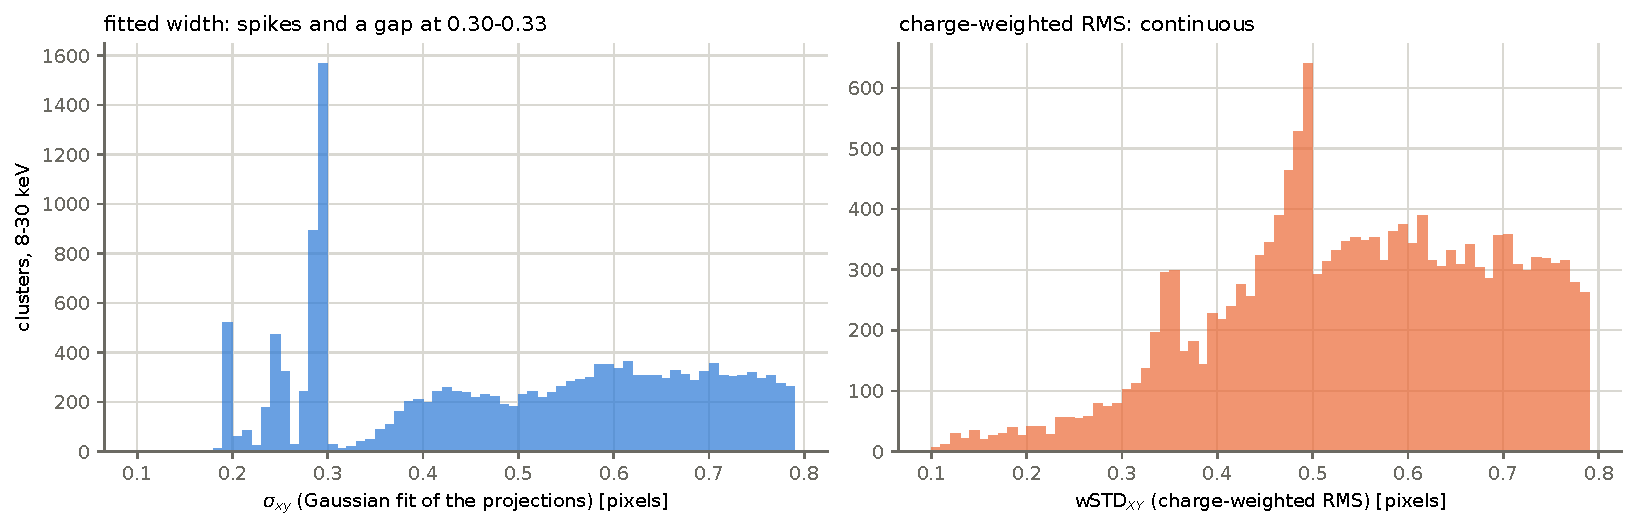
\includegraphics[width=0.9\textwidth]{figures/width_quantisation.pdf}
\caption{Width of 8--30\,keV clusters on EXT4: fitted $\sxy$ (left) and the charge-weighted RMS (right).}
\label{fig:quant}
\end{figure}

\subsection{Optimisation}
Cuts on the following variables were tried: upper and lower limits on $\sxy$ and \texttt{wSTD\_XY}, the fraction of
the cluster charge in its brightest pixel, the number of pixels, PCA elongation and linearity, the distance to the
nearest cluster, and the position on the CCD. Only the width helps; the charge fraction and number of pixels add
nothing beyond it, and line and continuum clusters look the same in shape, isolation and position.

A figure of merit from counts in fixed windows did not reproduce between independent halves of the data. The cuts
were therefore scored with the constrained fit itself: the combined significance of the four main line groups,
\begin{equation}
Z_\mathrm{Np} = \sqrt{Z_{\mathrm{L}\alpha}^2+Z_{\mathrm{L}\beta}^2+Z_{\mathrm{L}\gamma}^2+Z_{26.3}^2},
\qquad Z_g = A_g/\delta A_g ,
\end{equation}
on a grid of lower limits (0--0.5) and upper limits (0.6--0.9), separately on the even- and odd-numbered images
(Fig.~\ref{fig:band}, Table~\ref{tab:band}). $\sxy<0.7$ gives the highest significance on both halves.
A lower limit does not help: $0.2\le\sxy<0.7$ is equivalent to $\sxy<0.7$, and higher lower limits only remove
L-line clusters (the most compact clusters carry the cleanest L lines). Some loose bands reach a high $Z_\mathrm{Np}$
on all images but not on the halves, and have a poor deviance; these are unstable fits, not better cuts.
Figure~\ref{fig:spectra} shows the effect of the chosen cut on the whole spectrum.

\begin{figure}[H]
\centering
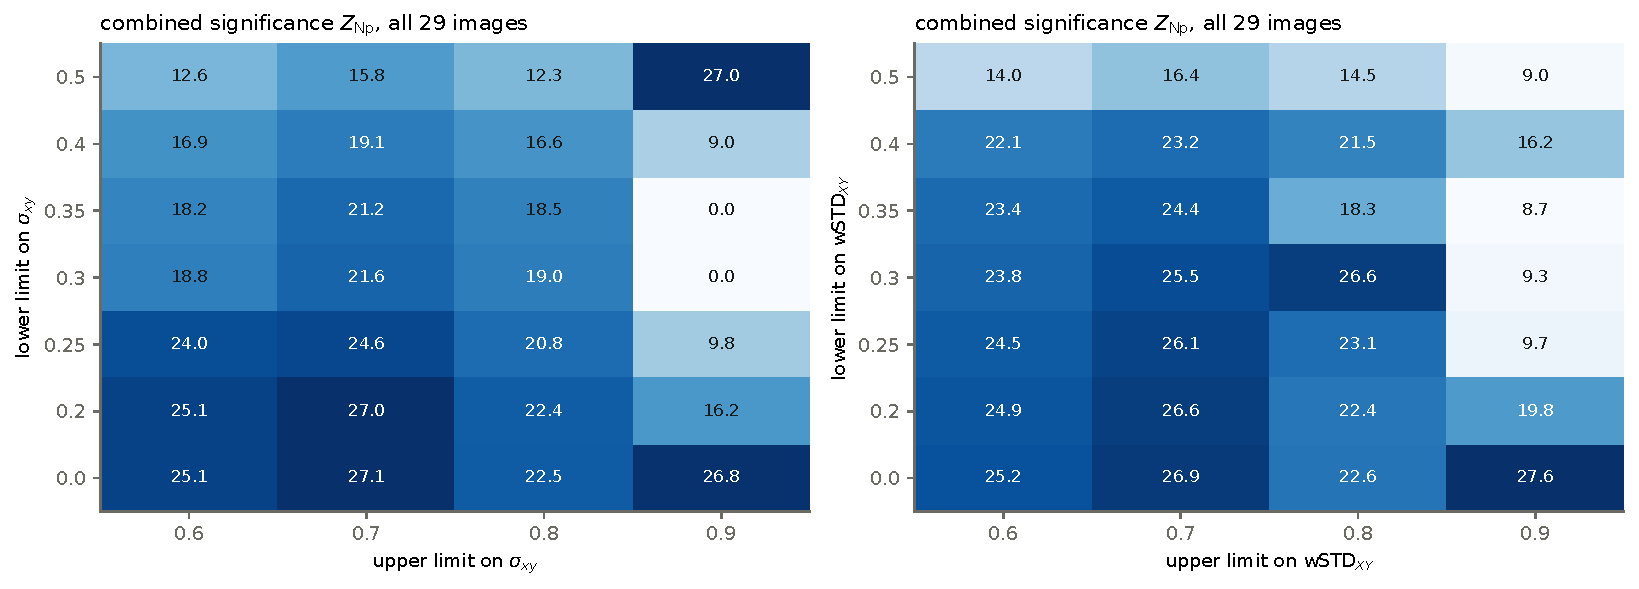
\includegraphics[width=\textwidth]{figures/band_grid.pdf}
\caption{Combined significance $Z_\mathrm{Np}$ of the constrained fit (EXT4, all 29 images) for bands
lower $\le$ width $<$ upper, for $\sxy$ (left) and \texttt{wSTD\_XY} (right).}
\label{fig:band}
\end{figure}

\begin{table}[H]
\centering
\caption{Selected width bands: clusters kept, $Z_\mathrm{Np}$ on all images and on the even/odd halves, energy
scale and deviance/ndf of the fit. 0.0 means the fit did not converge.}
\label{tab:band}
\begin{adjustbox}{max width=\textwidth}
\begin{tabular}{lcccccc}
\toprule
band & clusters & $Z_\mathrm{Np}$ & even & odd & $k$ & dev/ndf \\
\midrule
\tabinput{tables/band_grid_selected.tex}
\bottomrule
\end{tabular}
\end{adjustbox}
\end{table}

\begin{figure}[H]
\centering
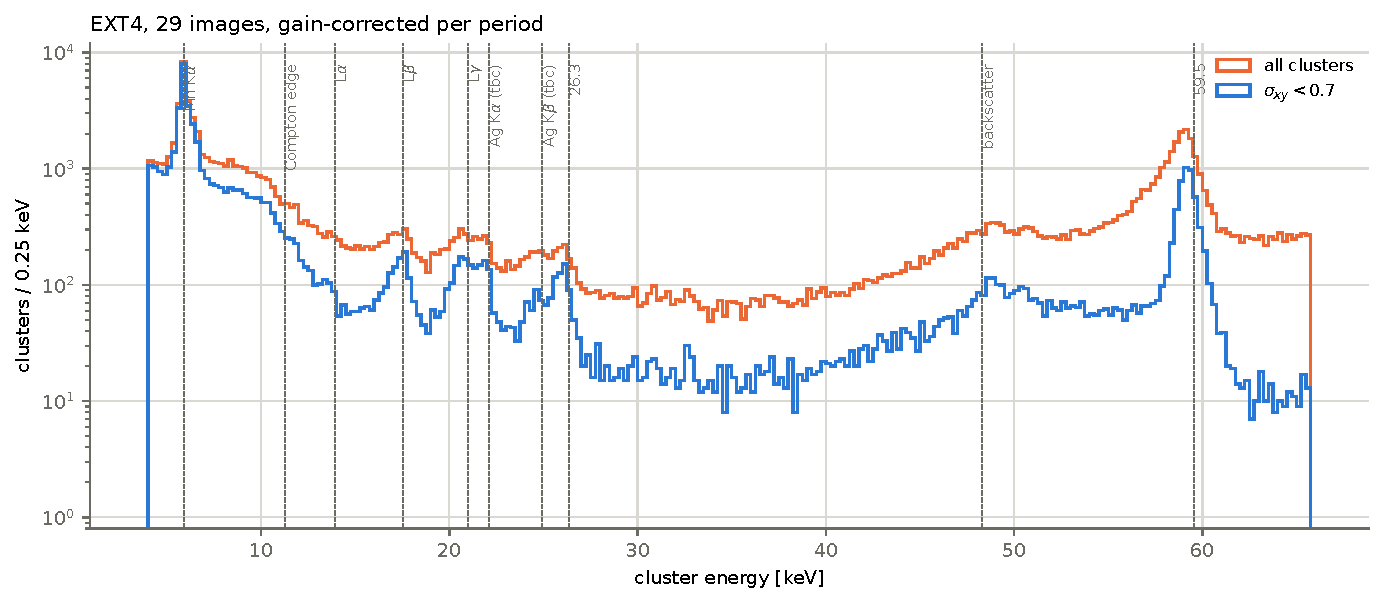
\includegraphics[width=\textwidth]{figures/spectra_cut.pdf}
\caption{EXT4 spectrum, all clusters and after $\sxy<0.7$ (gain-corrected per period). The cut removes most of the
continuum between 26 and 58\,keV and under the L lines, while the L lines, the 26.3\,keV line and the Fe-55 lines
survive.}
\label{fig:spectra}
\end{figure}

%======================================================================
\section{Constrained fit of the 10--30\,keV region}
\label{sec:fit}
\subsection{Model}
The expected counts in a bin of width $\Delta=0.2\keV$ centred at $E$ are
\begin{equation}
\mu(E) = b_0 + b_1(E-20) + b_2(E-20)^2
+ \frac{A_C}{2}\,\mathrm{erfc}\!\left(\frac{E-k\,E_C}{\sqrt2\,s_C}\right)
+ \sum_g A_g \sum_{i\in g} r_i\,\frac{\Delta}{\sqrt{2\pi}\,\sigma_i}
\exp\!\left[-\frac{(E-kE_i)^2}{2\sigma_i^2}\right],
\end{equation}
with
\begin{itemize}
\item $E_i$ the tabulated line energies and $r_i$ the relative intensities within group $g$ (normalised to 1), so
$A_g$ is the total number of counts in the group;
\item one energy scale $k$ for all lines (no individual shifts), so the fit cannot move neighbouring lines
independently;
\item widths $\sigma_i^2 = s_0^2 + s_1\,kE_i$ (noise and charge-statistics terms);
\item a quadratic background and a smeared step at the Compton edge of the 59.54\,keV $\gamma$ ray,
$E_C = E_\gamma\,\frac{2E_\gamma}{m_ec^2+2E_\gamma} = 11.25\keV$ for $E_\gamma=59.54\keV$.
\end{itemize}
The 15 free parameters are $k$, $s_0$, $s_1$, $b_{0,1,2}$, $A_C$, $s_C$ and the seven group totals $A_g$.

\subsection{Line list}
The Np L lines are those of L\'epy, Plagnard and Ferreux~\cite{lepy2008}, Table~3: 22 lines with their energies and
absolute emission probabilities, grouped as L$\ell$ (with L$t$, L$s$), L$\alpha$, L$\eta$, L$\beta$ (9 lines) and
L$\gamma$ (7 lines); within a group the relative intensities are fixed to the emission probabilities
(Table~\ref{tab:lines}). Where Table~3 gives one probability for two lines (L$\beta$ + L$\beta_5$ at 17.27/17.50\,keV,
L$\gamma_8$ + L$\gamma_3$ at 21.26/21.34\,keV) the pair is placed at the midpoint. The 26.34\,keV $\gamma$ ray of Am-241
is one more group (emission probability 2.31(8)\,\% in the evaluated decay data~\cite{ddep}, 2.40(3)\,\% in
L\'epy et al.; the fit uses only its energy). Two additional lines are required by the data; they are attributed to
silver K fluorescence, to be confirmed (Sec.~\ref{sec:extra}), and modelled with the Ag K-line energies: K$\alpha_1$ (22.16\,keV) and K$\alpha_2$ (21.99\,keV) with weights 2:1, and K$\beta_1$ (24.94\,keV) at
0.20 of K$\alpha$~\cite{xdb}; Ag K$\beta_2$ (about 25.46\,keV) is not included. L\'epy et al.\ quote the silicon K-escape peaks above 10\,keV at less
than $10^{-3}$ of the main peak; they are neglected.

\subsection{Likelihood, uncertainties and goodness of fit}
The parameters maximise the binned Poisson likelihood, i.e.\ minimise
$-\ln L = \sum_j \left[\mu_j - n_j \ln\mu_j\right]$ over the 100 bins $j$ with $n_j$ observed clusters.
Uncertainties are from the inverse of the numerical Hessian of $-\ln L$ at the minimum; uncertainties of derived
quantities (peak means, widths, FWHM, counts) are propagated with the full covariance matrix. The goodness of fit is
the deviance per degree of freedom,
\begin{equation}
\frac{D}{\mathrm{ndf}} = \frac{2}{N_\mathrm{bins}-N_\mathrm{par}}\sum_j\left[\mu_j-n_j+n_j\ln\frac{n_j}{\mu_j}\right],
\end{equation}
which is about 1 for a model that describes the data within Poisson fluctuations. The significance of a line group
is $Z_g = A_g/\delta A_g$: its fitted counts in units of their uncertainty.

\subsection{Pulls}
\label{sec:pulls}
The lower panel of Fig.~\ref{fig:fit} shows the pull of each bin,
\begin{equation}
p_j = \frac{n_j-\mu_j}{\sqrt{\mu_j}},
\end{equation}
the difference between data and fit in units of the expected Poisson fluctuation. If the model is right, the pulls
are independent and scatter like a unit Gaussian: mean 0, RMS 1, about 95\,\% within $\pm2$, and no runs of the same
sign. Isolated large pulls are fluctuations; several neighbouring pulls of the same sign mean the model misses a
feature there. For the fit of Fig.~\ref{fig:fit} the pulls have mean $-0.001$ and RMS 1.22 (85\,\% within $\pm2$;
RMS$^2\approx\chi^2/\mathrm{ndf} = 1.75$). The one clear structure is a run of positive pulls from 24.0 to 25.2\,keV
(+0.7 to +2.8), at and just above the Ag K$\beta$ line: fitted with free sizes the two silver lines have a ratio of
$0.49\pm0.07$, not the 0.20 fixed in this fit (Sec.~\ref{sec:extra}). Smaller alternating pulls at
10--11.5\,keV follow the Compton edge, whose shape is only approximately an error function.

\subsection{Results}
\begin{figure}[H]
\centering
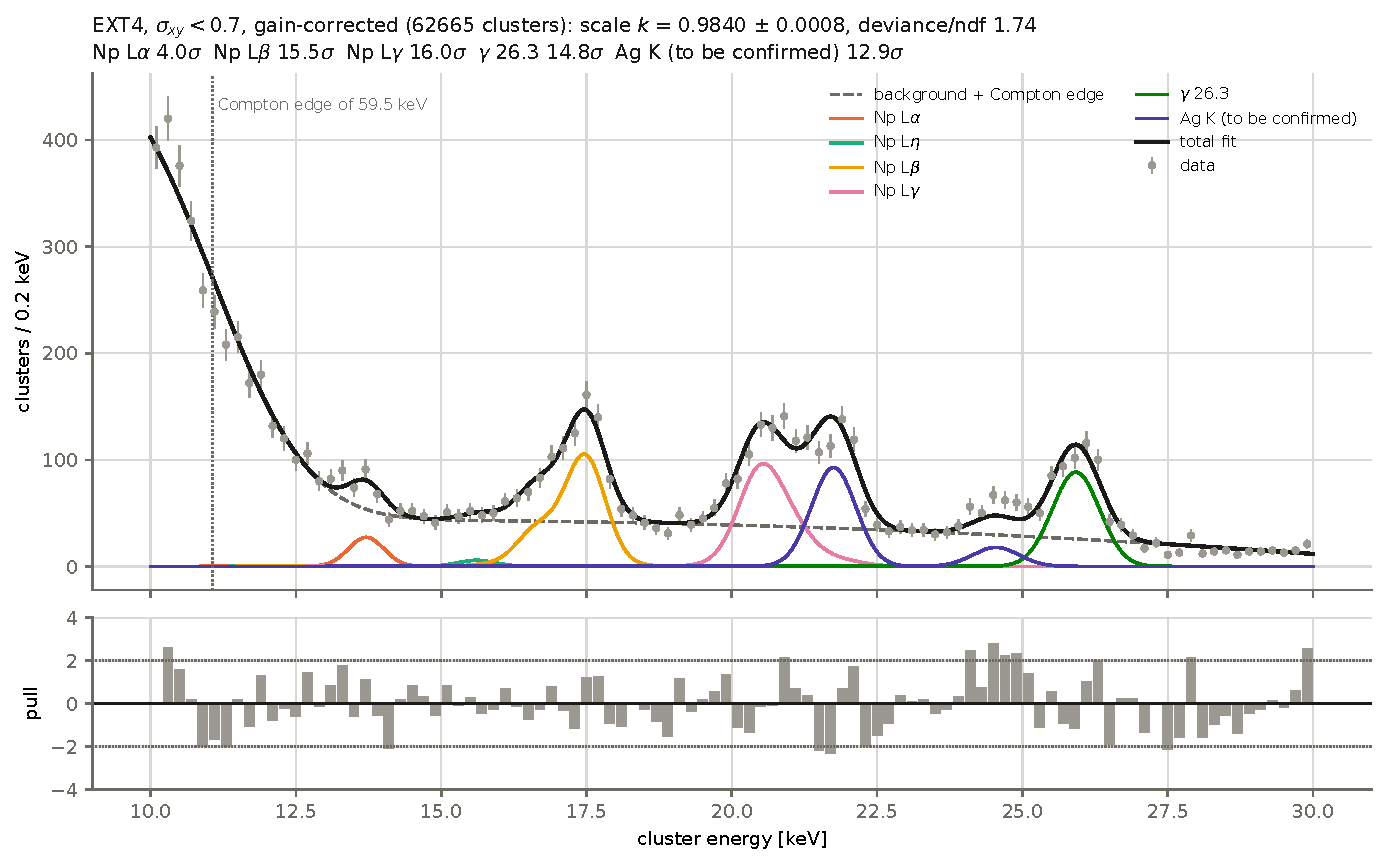
\includegraphics[width=\textwidth]{figures/fit_10_30.pdf}
\caption{\textbf{Figure of merit.} EXT4, $\sxy<0.7$, gain-corrected per gain period, 29 images. Points: data with
Poisson errors; black: total fit; dashed: background including the Compton step; coloured: the line groups. The
title gives the energy scale, the deviance/ndf and the significance of each group. Lower panel: pulls.}
\label{fig:fit}
\end{figure}

\begin{table}[H]
\centering
\caption{Fit parameters of Fig.~\ref{fig:fit}. $s_0$ is at its lower limit (0.05\,keV), so the widths are set by
$s_1$: $\sigma(E)\approx\sqrt{s_1E}$. Uncertainties are statistical; with deviance/ndf of 1.74 multiply them by about
$\sqrt{1.74}=1.32$ for a conservative estimate.}
\label{tab:fitpar}
\begin{adjustbox}{max width=\textwidth}
\begin{tabular}{lc}
\toprule
parameter & value \\
\midrule
\tabinput{tables/fit_parameters.tex}
\bottomrule
\end{tabular}
\end{adjustbox}
\end{table}

\begin{table}[H]
\centering
\caption{Fitted peaks of Fig.~\ref{fig:fit}. True centroid: intensity-weighted mean of the tabulated energies of the
group. Mean: fitted centroid ($k$ times the true centroid). $\sigma$: effective width (second moment of the group,
including the spread of its lines). FWHM: measured on the summed curve of the group. Counts: fitted counts in the
group. $Z$: significance $A_g/\delta A_g$. Ag K$\alpha$/K$\beta$: identification to be confirmed
(Sec.~\ref{sec:extra}); fitted with the Ag K energies (their ``true'' values) and a fixed 0.20 ratio, sharing one
amplitude. With free sizes they have
$408\pm33$ and $202\pm24$ counts (Table~\ref{tab:extra}).}
\label{tab:groups}
\small
\begin{adjustbox}{max width=\textwidth}
\begin{tabular}{lccccccc}
\toprule
peak & true [keV] & mean [keV] & mean/true & $\sigma$ [keV] & FWHM [keV] & counts & $Z$ \\
\midrule
\tabinput{tables/groups.tex}
\bottomrule
\end{tabular}
\end{adjustbox}
\end{table}

The L$\beta$ and L$\gamma$ groups are wider ($\sigma\approx0.53\keV$) than their FWHM/2.355 ($\approx0.42$--$0.46\keV$)
because their weaker lines (L$\beta_2$, L$\beta_4$ at 16.8--17.1\,keV; L$\gamma_2$--L$\gamma_6$ at 21.1--21.5\,keV)
add shoulders that widen the group without raising its maximum; the maximum of L$\beta$ is at L$\beta_1$
($17.466\keV$). Np L$\ell$ sits on the Compton edge and is not separated from it; L$\eta$ is not significant.
The individual lines are in Table~\ref{tab:lines} (Appendix).

\paragraph{Without the gain correction} the same fit gives $k = 0.9358\pm0.0008$: all lines 6.4\,\% low, with similar
significances, since the correction mainly rescales the energies.

\paragraph{Without the width cut} the fit cannot separate the lines (Fig.~\ref{fig:fitall}): the scale drops to
$k=0.966$, the deviance/ndf rises to 2.24, and the covariance matrix is singular for all groups except the
26.3\,keV $\gamma$ ray.

\begin{figure}[H]
\centering
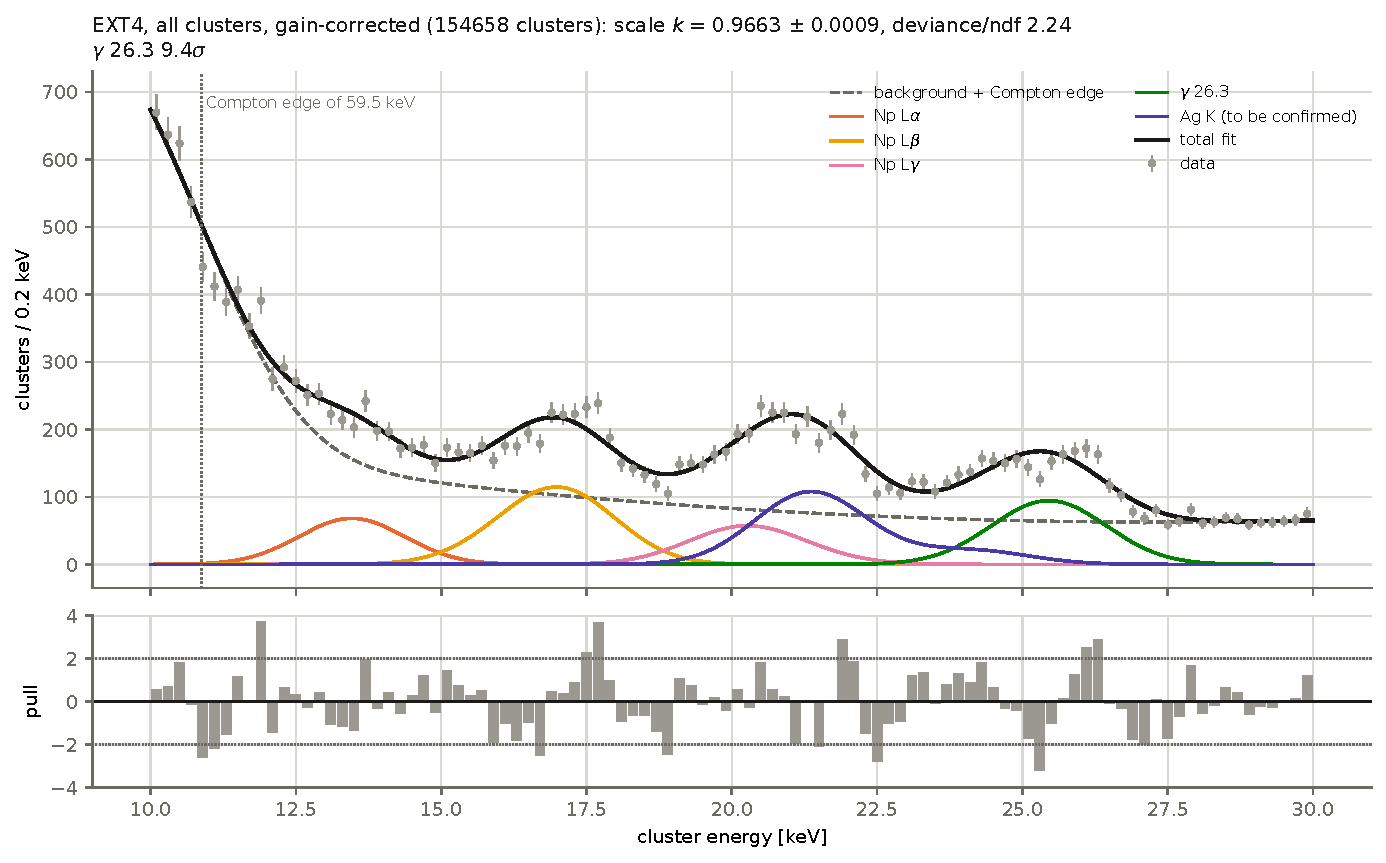
\includegraphics[width=\textwidth]{figures/fit_10_30_allclusters.pdf}
\caption{The same fit with all clusters (no width cut). The L groups merge into the continuum; only the 26.3\,keV
line has a defined uncertainty.}
\label{fig:fitall}
\end{figure}

\subsection{Silver K lines at 22.1 and 24.9\,keV (to be confirmed)}
\label{sec:extra}
The Np L lines and the 26.3\,keV $\gamma$ ray alone, with the intensity ratios of L\'epy et al., do not describe the
data ($-2\Delta\ln L = 294.7$ and deviance/ndf 4.81 against the best model, Table~\ref{tab:hyp}). Two additional lines
are needed. Fitted with a free energy and size each (on the common energy scale $k$), they are at
$22.112\pm0.037\keV$ and $24.933\pm0.060\keV$ with $408\pm33$ and $202\pm24$ counts (Table~\ref{tab:extra}).
\textbf{We attribute them to silver K fluorescence, to be confirmed}, and model them with the Ag K-line energies in
the main fit (Fig.~\ref{fig:fit}). The hypotheses examined so far are listed below and in Table~\ref{tab:hyp}.

\begin{table}[H]
\centering
\caption{The two additional lines fitted with free energy and size (EXT4, $\sxy<0.7$, gain-corrected, 29 images).
True energy: observed energy divided by the common scale $k$ of the Np lines.}
\label{tab:extra}
\begin{adjustbox}{max width=\textwidth}
\begin{tabular}{lccc}
\toprule
 & observed [keV] & true [keV] & counts \\
\midrule
\tabinput{tables/extra_lines.tex}
\bottomrule
\end{tabular}
\end{adjustbox}
\end{table}

\paragraph{Am-241 photons.} The evaluated decay data~\cite{ddep} list no Am-241 x ray or $\gamma$ ray between the
end of the Np L series (22.2\,keV) and the 26.34\,keV $\gamma$ ray. The silicon K-escape peak of the 26.3\,keV line
(24.60\,keV) is below $10^{-3}$ of the line~\cite{lepy2008}, far too weak, and 5$\sigma$ from the fitted 24.93\,keV.

\paragraph{Np L$\gamma_4$ (downshifted, enhanced).} Np L$\gamma_4$ (22.12\,keV) sits exactly at the energy of the first
line once the common energy scale is applied (observed 21.77\,keV). With the Table~3 ratios it contributes only about
24 counts; the data would need it about 18 times stronger. A fit with free L$\gamma_4$/L$\gamma_{13}$ sizes plus a
free line for the 24.9\,keV structure describes the data almost as well as two free lines ($-2\Delta\ln L = 4.2$).
However, L$\gamma_4$ is an L1-subshell transition: L$\gamma_4$, L$\gamma_{13}$, L$\beta_3$ and L$\beta_4$ all fill L1
vacancies, so their intensity ratios are fixed by atomic transition rates, and an 18-fold L$\gamma_4$ would require
equally enhanced L$\beta_4$ and L$\beta_3$. With all four free the fit finds no excess at L$\beta_4$ or L$\beta_3$
(Table~\ref{tab:l1}). Absorption in the source material cannot single out L$\gamma_4$ either: it lies above the
Np L2 absorption edge (21.60\,keV) and would be absorbed more, not less, than L$\gamma_1$. An enhanced L$\gamma_4$ also
leaves the 24.9\,keV line unexplained. Our tests therefore disfavour this hypothesis.

\begin{table}[H]
\centering
\caption{L1-subshell lines: size from the Table~3 ratios (scaled to the fitted L$\beta$/L$\gamma$ groups), the size
needed if all L1 lines were enhanced as much as L$\gamma_4$ would have to be (factor 18), and the extra counts fitted
when the four lines are free (plus a free line at 24.9\,keV). L$\gamma_4$ and L$\gamma_{13}$ are 0.28\,keV apart and
not separated by the fit.}
\label{tab:l1}
\begin{adjustbox}{max width=\textwidth}
\begin{tabular}{lcccc}
\toprule
line & $E$ [keV] & tabulated [counts] & if enhanced $\times18$ & fitted extra [counts] \\
\midrule
\tabinput{tables/l1_lines.tex}
\bottomrule
\end{tabular}
\end{adjustbox}
\end{table}

\paragraph{Am L self-fluorescence.} L\'epy et al.\ label americium L lines excited in the source itself (Am
L$\alpha$ 14.41/14.62, L$\beta_{2,15}$ 17.66, L$\beta_1$ 18.86, L$\gamma_1$ 22.07\,keV). Am L$\gamma_1$ matches the
first line, but with the five Am lines free the fit puts $356\pm33$ counts in Am L$\gamma_1$ and $0\pm5$ in Am
L$\beta_1$, while in an L spectrum L$\beta_1$ is several times stronger than L$\gamma_1$ (four times for Np). It also
does not produce the 24.9\,keV line. Disfavoured.

\paragraph{Conversion electrons.} The decay data~\cite{ddep} list conversion electrons in exactly this range:
ec$_{4,2}$L (20.99--25.81\,keV), ec$_{2,1}$M (20.61--22.68\,keV) and ec$_{3,1}$L (20.28--25.09\,keV), 12.8 per
100 decays in total. If electrons from the source reached the CCD, the much stronger ec$_{2,0}$L line (37.11, 37.94,
41.93\,keV; 30.2 per 100 decays) would appear with at least about 1400 counts (more if material between source and
CCD stops the slower electrons first). The fit finds $26\pm26$ counts (Table~\ref{tab:ce}). Excluded.

\begin{table}[H]
\centering
\caption{Conversion-electron test. First row: the electron lines at 20.3--25.8\,keV and the counts of the
two extra lines (22.1 and 24.9\,keV) that they would have to account for. Second row: expected counts in the
ec$_{2,0}$L line if they did, scaled by the electron intensities~\cite{ddep}. Fitted: Poisson fit of 33--46\,keV with Gaussians at the
three ec$_{2,0}$L energies (EXT4, $\sxy<0.7$).}
\label{tab:ce}
\begin{adjustbox}{max width=\textwidth}
\begin{tabular}{lcccc}
\toprule
electron line & energies [keV] & per 100 decays & expected [counts] & fitted [counts] \\
\midrule
\tabinput{tables/conversion_electrons.tex}
\bottomrule
\end{tabular}
\end{adjustbox}
\end{table}

\paragraph{Sn K fluorescence.} K$\alpha$ at 25.04/25.27\,keV, K$\beta$ at 28.49\,keV: does not match
($-2\Delta\ln L = 267.7$).

\paragraph{Ag K fluorescence (adopted, to be confirmed).} Both energies agree within one standard deviation with silver:
Ag K$\alpha$ (K$\alpha_1$/K$\alpha_2$ centroid 22.10\,keV) and Ag K$\beta_1$ (24.94\,keV)~\cite{xdb}. Silver near the
source or the CCD would be excited by the Am-241 $\gamma$ rays above the Ag K edge (25.5\,keV). We know of no other
element with K lines at both energies. The size ratio does not fit standard silver fluorescence, however: the two lines
have $0.49\pm0.07$, while the Ag K$\beta$/K$\alpha$ ratio is about 0.2 (about 0.27 after the rise of the detection
efficiency with energy estimated from our 26.3\,keV/L$\gamma$ ratio), a tension of about three standard deviations.
With the ratio fixed to 0.20 the fit is worse than with free sizes ($-2\Delta\ln L = 29.2$) and leaves the positive
pulls at 24--25\,keV.

\paragraph{Source construction.} The Am-241 source comes from a French ionisation smoke detector. The americium foils
of such detectors are commonly made of americium oxide in a gold matrix on a silver backing, with a thin gold or
gold--palladium cover; the construction of this particular source has not been checked. If it is of this type, silver
sits directly behind the americium and is irradiated by the 59.54\,keV $\gamma$ rays, which would produce Ag K
fluorescence naturally. Absorption of Ag K$\alpha$ (22.1\,keV) relative to K$\beta$ (24.9\,keV) in a thick silver
backing and in the gold layer would also raise the observed K$\beta$/K$\alpha$ ratio above 0.2, possibly up to the
measured 0.49; this has not been calculated. Gold L x rays (9.7--13.4\,keV) would be expected too. Local fits find no
Au L$\alpha$ (9.71\,keV) or L$\beta$ (11.44/11.58\,keV) peak, but the data show strong suppression at low energy
(Np L$\alpha$ at about a quarter of its tabulated size relative to L$\beta$), so their absence is not conclusive.

\paragraph{Status.} The two lines are significant and do not come from the Am-241 decay. They are labelled as silver
K lines, to be confirmed: silver is the only candidate found that matches both energies, and smoke-detector
americium foils commonly have a silver backing; the intensity ratio is not yet explained quantitatively; something else, such as an enhanced Np L$\gamma_4$, was also considered, though the tests above
disfavour it. Next checks: the construction of the source (manufacturer or foil specification) and the materials near the
source and the CCD; a calculation of the K$\beta$/K$\alpha$ ratio for a silver-backed, gold-covered foil; whether the
two lines have the same distribution over the CCD as the Np lines; data with the source moved or shielded; and a fit
with the K$\beta$/K$\alpha$ ratio free and Ag K$\beta_2$ included.

\begin{table}[H]
\centering
\caption{Hypotheses for the two additional lines (EXT4, $\sxy<0.7$, gain-corrected, 29 images): number of free
parameters, $-2\ln L$ relative to the best model, and deviance/ndf. ``Free line'': a Gaussian with free energy and size.}
\label{tab:hyp}
\small
\begin{adjustbox}{max width=\textwidth}
\begin{tabular}{lccc}
\toprule
model & parameters & $-2\Delta\ln L$ & dev/ndf \\
\midrule
\tabinput{tables/hypotheses.tex}
\bottomrule
\end{tabular}
\end{adjustbox}
\end{table}

%======================================================================
\section{Other peaks}
\label{sec:other}
Table~\ref{tab:other} and Fig.~\ref{fig:other} give the peaks outside 10--30\,keV, fitted separately with a free
mean and width each, for all clusters and after the cut (EXT4, gain-corrected per period).
\begin{itemize}
\item \textbf{59.54\,keV $\gamma$ ray}: Gaussian plus linear background, fitted from 1.2\,keV below to 1.5\,keV above
the maximum (the low-energy tail from incomplete charge collection is left out). At 0.994 of the true energy after
the cut.
\item \textbf{Backscatter peak}: 59.54\,keV $\gamma$ rays that scatter in material around the CCD and are absorbed in
it. A photon scattered by $180^\circ$ keeps $E_\gamma - E_C = 48.3\keV$, the minimum; most backscatter is at smaller
angles, so the peak lies above 48.3\,keV ($49.28\pm0.13\keV$, 12$\sigma$ after the cut).
\item \textbf{Compton edge}: position of the error-function step in a 7.5--30\,keV fit with the edge position free.
The free-electron value is 11.25\,keV ($11.07\keV$ on the fitted scale $k$); the measured edge, $10.82\pm0.06\keV$
(after the cut) and smeared by $s_C\approx1.5\keV$, lies lower because the electrons in silicon are bound (Doppler
broadening) and because of the detector resolution.
\item \textbf{Fe-55 Mn K$\alpha$/K$\beta$} (5.899/6.490\,keV, common scale and width): an Fe-55 source is also
present. At 0.996 of the true energy, with $\sigma=0.158\keV$.
\end{itemize}

\begin{table}[H]
\centering
\caption{Peaks outside 10--30\,keV (EXT4, gain-corrected per period). For the Compton edge, ``$\sigma$'' is the
smearing $s_C$ of the step. $Z$: amplitude significance.}
\label{tab:other}
\small
\begin{adjustbox}{max width=\textwidth}
\begin{tabular}{lcccccc}
\toprule
peak & true [keV] & mean [keV] & mean/true & $\sigma$ [keV] & FWHM [keV] & $Z$ \\
\midrule
\tabinput{tables/other_peaks.tex}
\bottomrule
\end{tabular}
\end{adjustbox}
\end{table}

\begin{figure}[H]
\centering
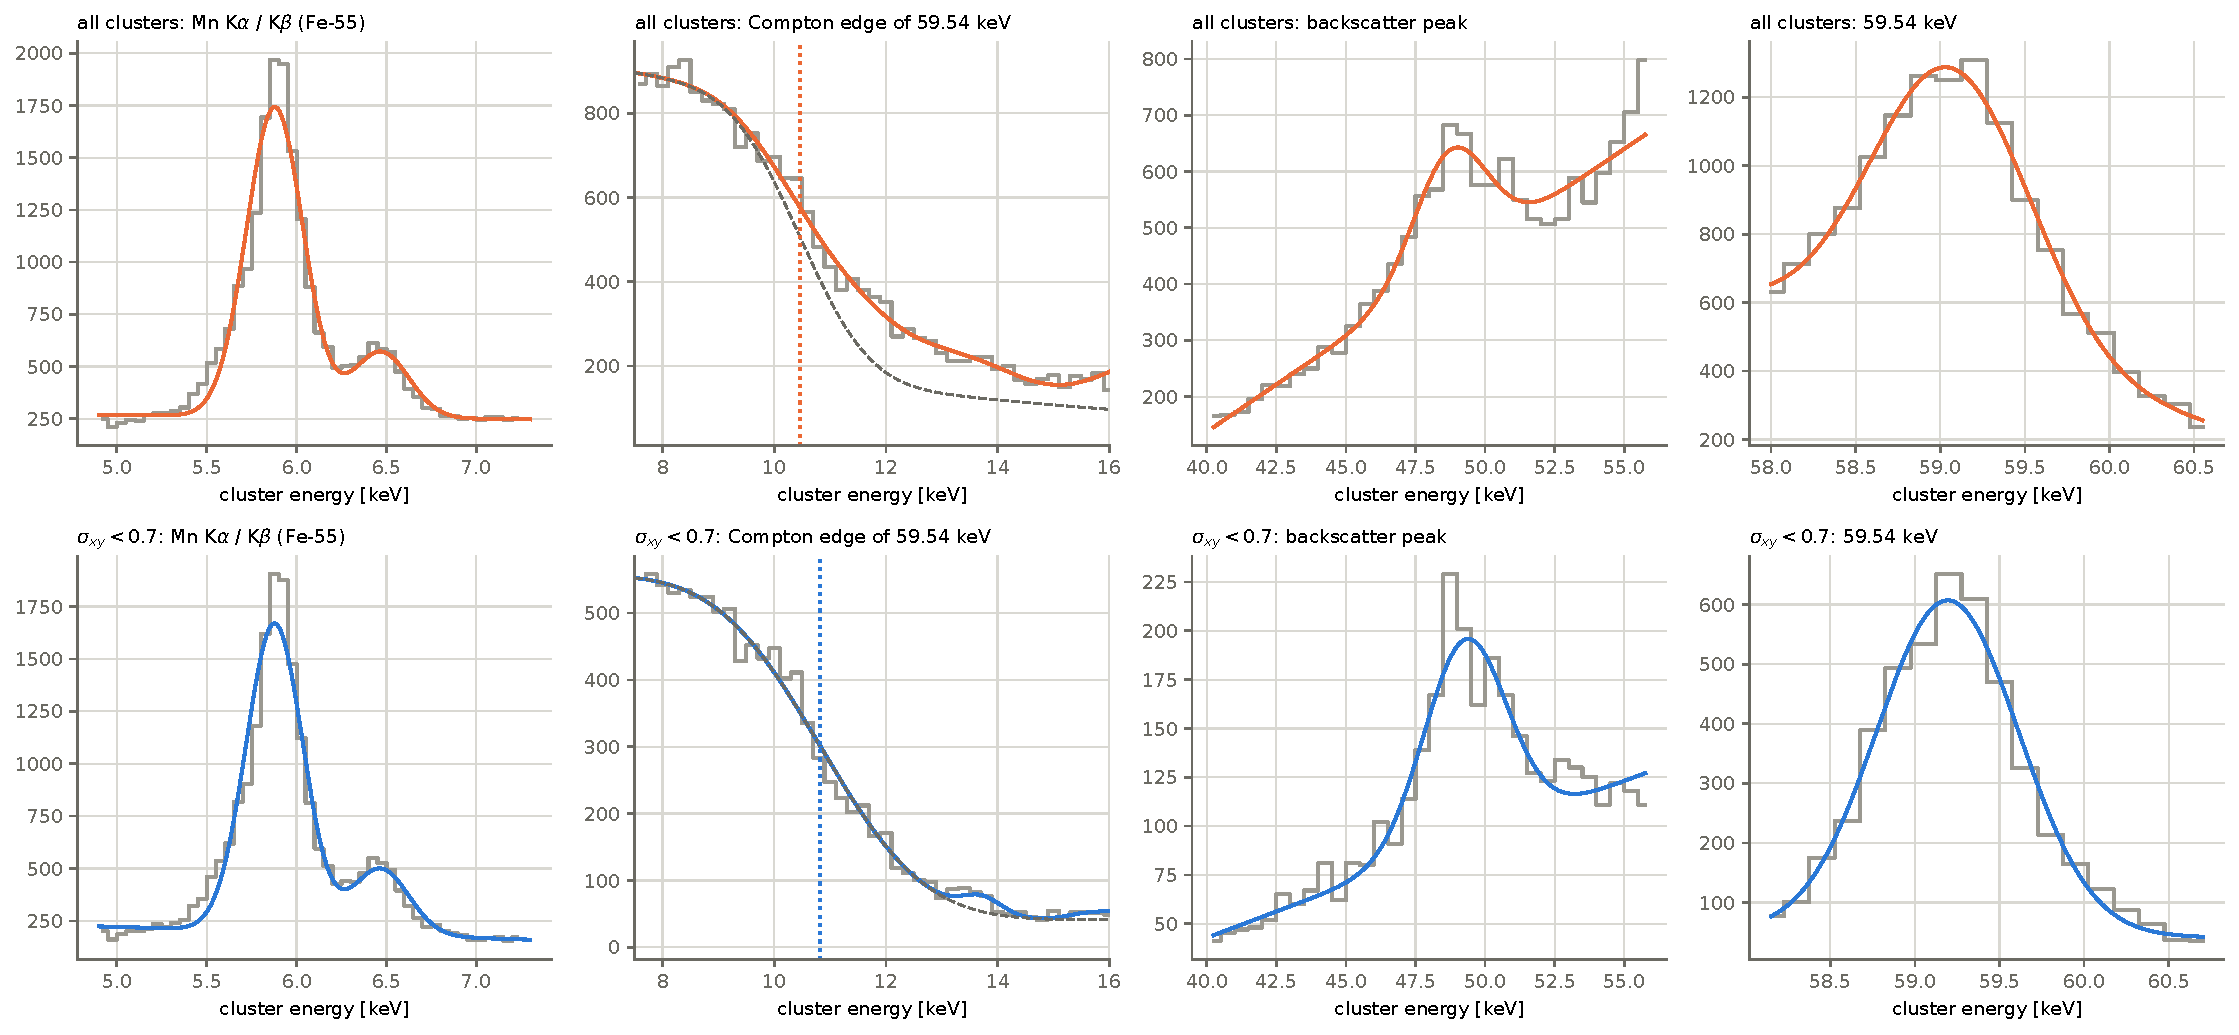
\includegraphics[width=\textwidth]{figures/other_peaks.pdf}
\caption{EXT4, gain-corrected: Fe-55 lines, Compton edge (dashed: background without the line groups), backscatter
peak and 59.54\,keV peak, for all clusters (top) and after $\sxy<0.7$ (bottom).}
\label{fig:other}
\end{figure}

%======================================================================
\section{How the gain correction and the width cut bring out the lines}
\begin{itemize}
\item \textbf{Gain correction} puts the peaks at the right energies (EXT4 59.54\,keV: $0.932\to0.992$;
10--30\,keV lines: $k = 0.936\to0.984$) and lines up all images (59.54\,keV peak scatter 0.25\,\% after correction).
Without it the per-image gain scatter smears every peak, and identifying lines by energy fails.
\item \textbf{One curve per gain period} is needed because the gain stepped by 1--5\,\% between images \#40 and
\#41; a single curve leaves the later images 3\,\% low and splits the summed peaks.
\item \textbf{The width cut} removes the continuum that buries the L lines. Without it the 10--30\,keV fit cannot
separate the lines; with $\sxy<0.7$ the L$\beta$, L$\gamma$, 26.3\,keV and Ag K (to be confirmed) groups
are found at 13--16$\sigma$
and L$\alpha$ at 4$\sigma$, and the fit describes the data to deviance/ndf 1.74.
\item \textbf{The constrained model} (tabulated energies and intensity ratios, one energy scale) makes the
overlapping groups separable and turns the spectrum into one energy-scale measurement, $k = 0.9840\pm0.0008$.
\end{itemize}

%======================================================================
\section{Limitations}
\begin{itemize}
\item Uncertainties are statistical. With deviance/ndf = 1.74 they should be enlarged by about 1.3.
\item After the gain correction the 10--30\,keV lines are still 1.6\,\% low, while the 59.54\,keV and Mn K$\alpha$
lines are 0.6 and 0.4\,\% low. Candidates: charge lost below the pixel threshold in compact high-charge clusters, and
the extrapolation of $g(n)$ above the measured range ($n_\mathrm{max} = 480$--$1130\,e^-$, while the brightest pixel
of a compact L-line cluster holds of order 3000\,e$^-$).
\item $s_0$ is at its lower limit; the width model is effectively $\sigma\propto\sqrt{E}$.
\item The identification of the 22.1 and 24.9\,keV lines as silver is to be confirmed (Sec.~\ref{sec:extra}). The
main fit models them with the Ag K energies and a fixed K$\beta$/K$\alpha$ ratio of 0.20, which the data do not support ($0.49\pm0.07$ with
free sizes); this causes the pulls at 24--25\,keV. The Mn line energies are standard values~\cite{xdb}.
\item The fitted group counts are not corrected for absorption in front of the CCD or for the efficiency of the width
cut, which both depend on energy; they cannot be compared directly with the emission probabilities.
\item EXT3 and EXT1 have too few L-line counts for a physical constrained fit; their 59.54\,keV, backscatter and
Mn K results are in the analysis tables.
\end{itemize}

%======================================================================
\section{Reproducing the analysis}
All paths are relative to \texttt{JH1\_Testing/AMTEst/runs\_29img/}. Pipeline (\texttt{comm\_scripts}, default
\texttt{--gain-model interpolated}):
\begin{verbatim}
run_WADERs AMtest_29.txt -o no_gaincorr --composite
run_WADERs AMtest_29.txt -o gaincorr --composite --gain-correction
\end{verbatim}
Gain curve per gain period: \texttt{gain\_vs\_charge.py measure} on images \#21--\#40 and \#41--\#50
(\texttt{--ext 1 3 4}), then \texttt{gain\_vs\_charge.py apply} on each period's cluster files; output in
\begin{verbatim}
gaincorr/WADERs_analysis_AMtest_29/root_gaincorr_epochs/
\end{verbatim}
Analysis scripts (folder \texttt{analysis/}):
\begin{itemize}
\item \texttt{load2.py}: cluster quantities from the cluster files;
\item \texttt{amfit.py}: the constrained 10--30\,keV model;
\item \texttt{fits29.py}: all fits and the band-cut grid;
\item \texttt{peak\_table.py}: peak parameters;
\item \texttt{figs\_doc.py}: the figures and tables of this note;
\item \texttt{test\_extra\_lines.py}, \texttt{test\_lgamma4.py}, \texttt{tab\_hypotheses.py}: identification tests of the
22.1/24.9\,keV lines;
\item \texttt{test\_gold.py}: gold L lines.
\end{itemize}

%======================================================================
\appendix
\section{Individual lines}
{\small\setlength{\tabcolsep}{4pt}
\begin{longtable}{lcccccc}
\caption{Every line of the fit of Fig.~\ref{fig:fit}. $E$ and $P$: tabulated energy and emission probability
per decay~\cite{lepy2008}. Ag K lines (t.b.c.\ = to be confirmed): the 22.1/24.9\,keV lines, fitted with the Ag K
energies~\cite{xdb} (Sec.~\ref{sec:extra}). Mean, $\sigma$, FWHM
and counts: from the fit, uncertainties propagated with the full covariance.}
\label{tab:lines}\\
\toprule
line & $E$ [keV] & $P$ [\%] & mean [keV] & $\sigma$ [keV] & FWHM [keV] & counts \\
\midrule
\endfirsthead
\toprule
line & $E$ [keV] & $P$ [\%] & mean [keV] & $\sigma$ [keV] & FWHM [keV] & counts \\
\midrule
\endhead
\tabinput{tables/lines.tex}
\bottomrule
\end{longtable}}

\begin{thebibliography}{9}
\bibitem{lepy2008} M.-C. L\'epy, J. Plagnard, L. Ferreux, \emph{Measurement of $^{241}$Am L X-ray emission
probabilities}, Appl.\ Radiat.\ Isot.\ \textbf{66} (2008) 715--721, doi:10.1016/j.apradiso.2008.02.078.
\bibitem{ddep} V.~P. Chechev, N.~K. Kuzmenko (KRI), evaluated decay data for $^{241}$Am (LNHB/DDEP
\emph{Table of Radionuclides}): $\alpha$, electron, x-ray and $\gamma$-ray emissions.
\bibitem{xdb} A.~C. Thompson et al., \emph{X-ray Data Booklet}, Lawrence Berkeley National Laboratory
(\url{https://xdb.lbl.gov}); Ag and Mn K line energies used here: Ag K$\alpha_1$ 22.16, K$\alpha_2$ 21.99,
K$\beta_1$ 24.94\,keV; Mn K$\alpha_1$ 5.899, K$\beta$ 6.490\,keV.
\end{thebibliography}

\end{document}
